%%% MORITZ 5' %%%

\section{Franzen}
\subsection{Grundlagen}
\begin{frame}
\frametitle{Grundlagen: Franzen}
  
\end{frame}

\subsection{Aufbau}
\begin{frame}
\frametitle{Aufbau: Franzen}

\setbeamerfont{myfont}{size*=80}
\usebeamerfont{myfont}
\begin{figure}
    \centering
    \def\svgwidth{\textwidth}
    \input{../img/aufbaufranzen.pdf_tex}
    \caption{Aufbau..}
\end{figure}
\usebeamerfont{standard}

\begin{itemize}
  \item \textbf{Chopper:} Periodische Unterbrechung des Laserlichts
  \item \textbf{Spule 1:} Kompensation von horizontalem Erdmagnetfeld
  \item \textbf{Spule 4:} Kompensation von vertikalem Erdmagnetfeld
\end{itemize}

\end{frame}

\subsection{Auswertung}
\begin{frame}
\frametitle{Auswertung: Franzen}

\begin{figure}
    \centering
    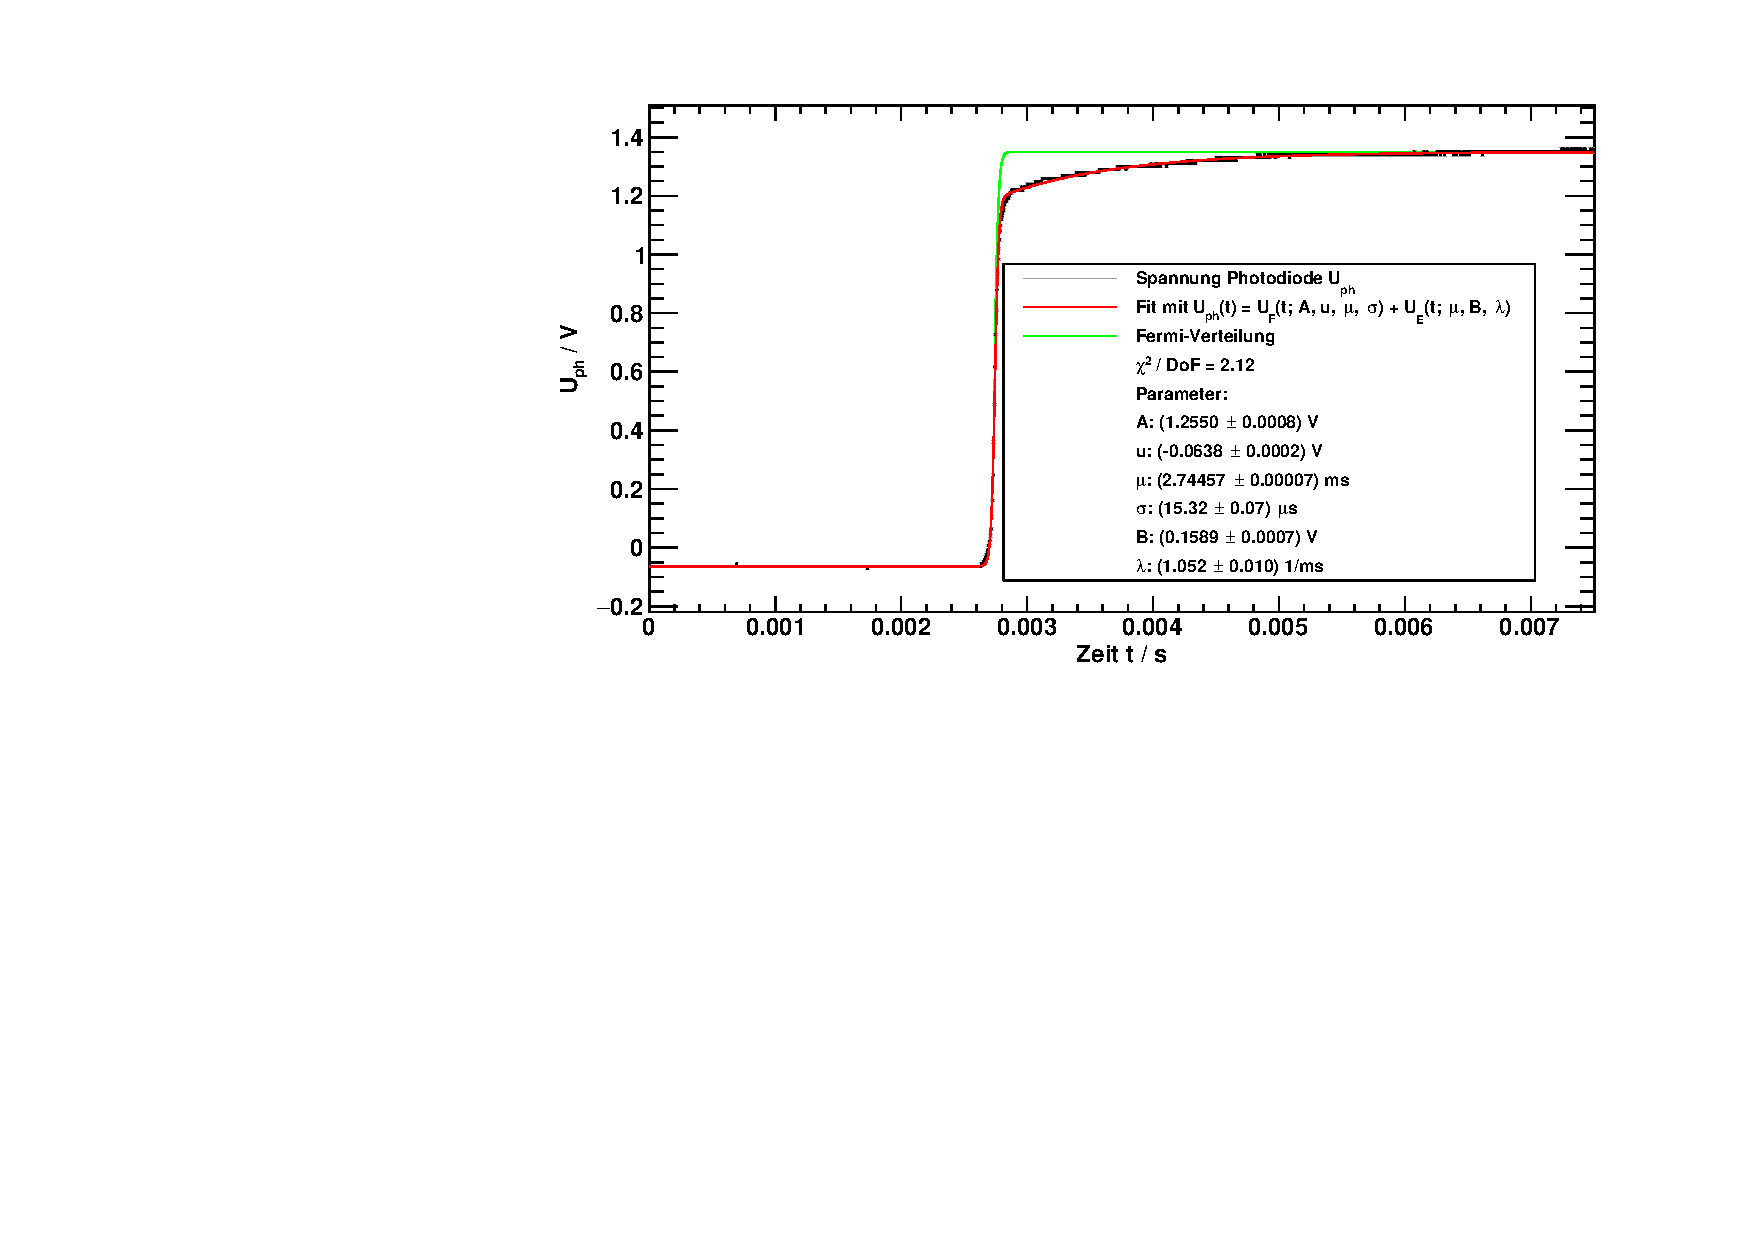
\includegraphics[width=\textwidth]{../img/04.pdf}
    \caption{Transmission der Messzelle nach Öffnung des Strahlengangs.}  
\end{figure} 
  
\end{frame}


\begin{frame}
\frametitle{Auswertung: Franzen}

\begin{figure}
    \centering
    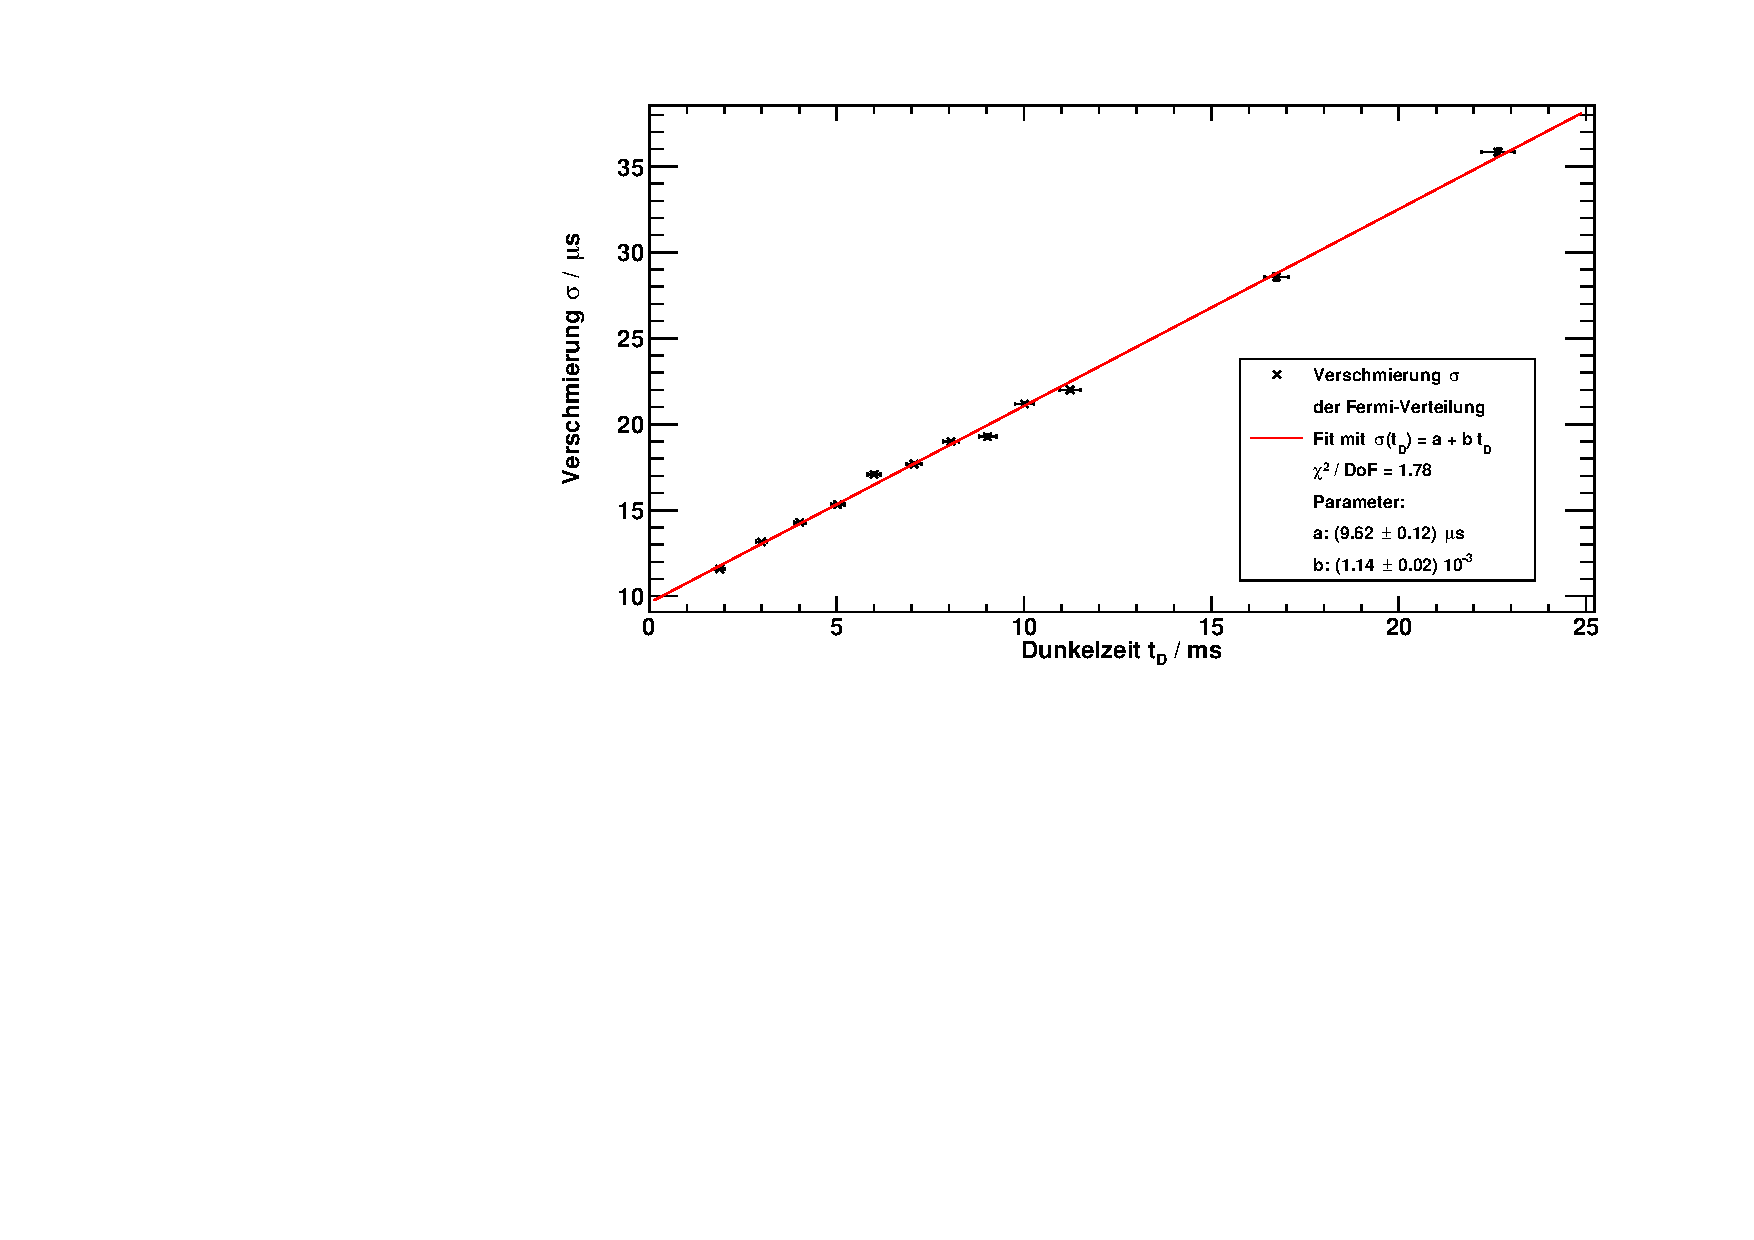
\includegraphics[width=\textwidth]{../img/sigmaFit.pdf}
    \caption{Abrundung der gefitteten Fermi-Funktionen.}  
\end{figure} 
  
\end{frame}


\begin{frame}
\frametitle{Auswertung: Franzen}

\begin{figure}
    \centering
    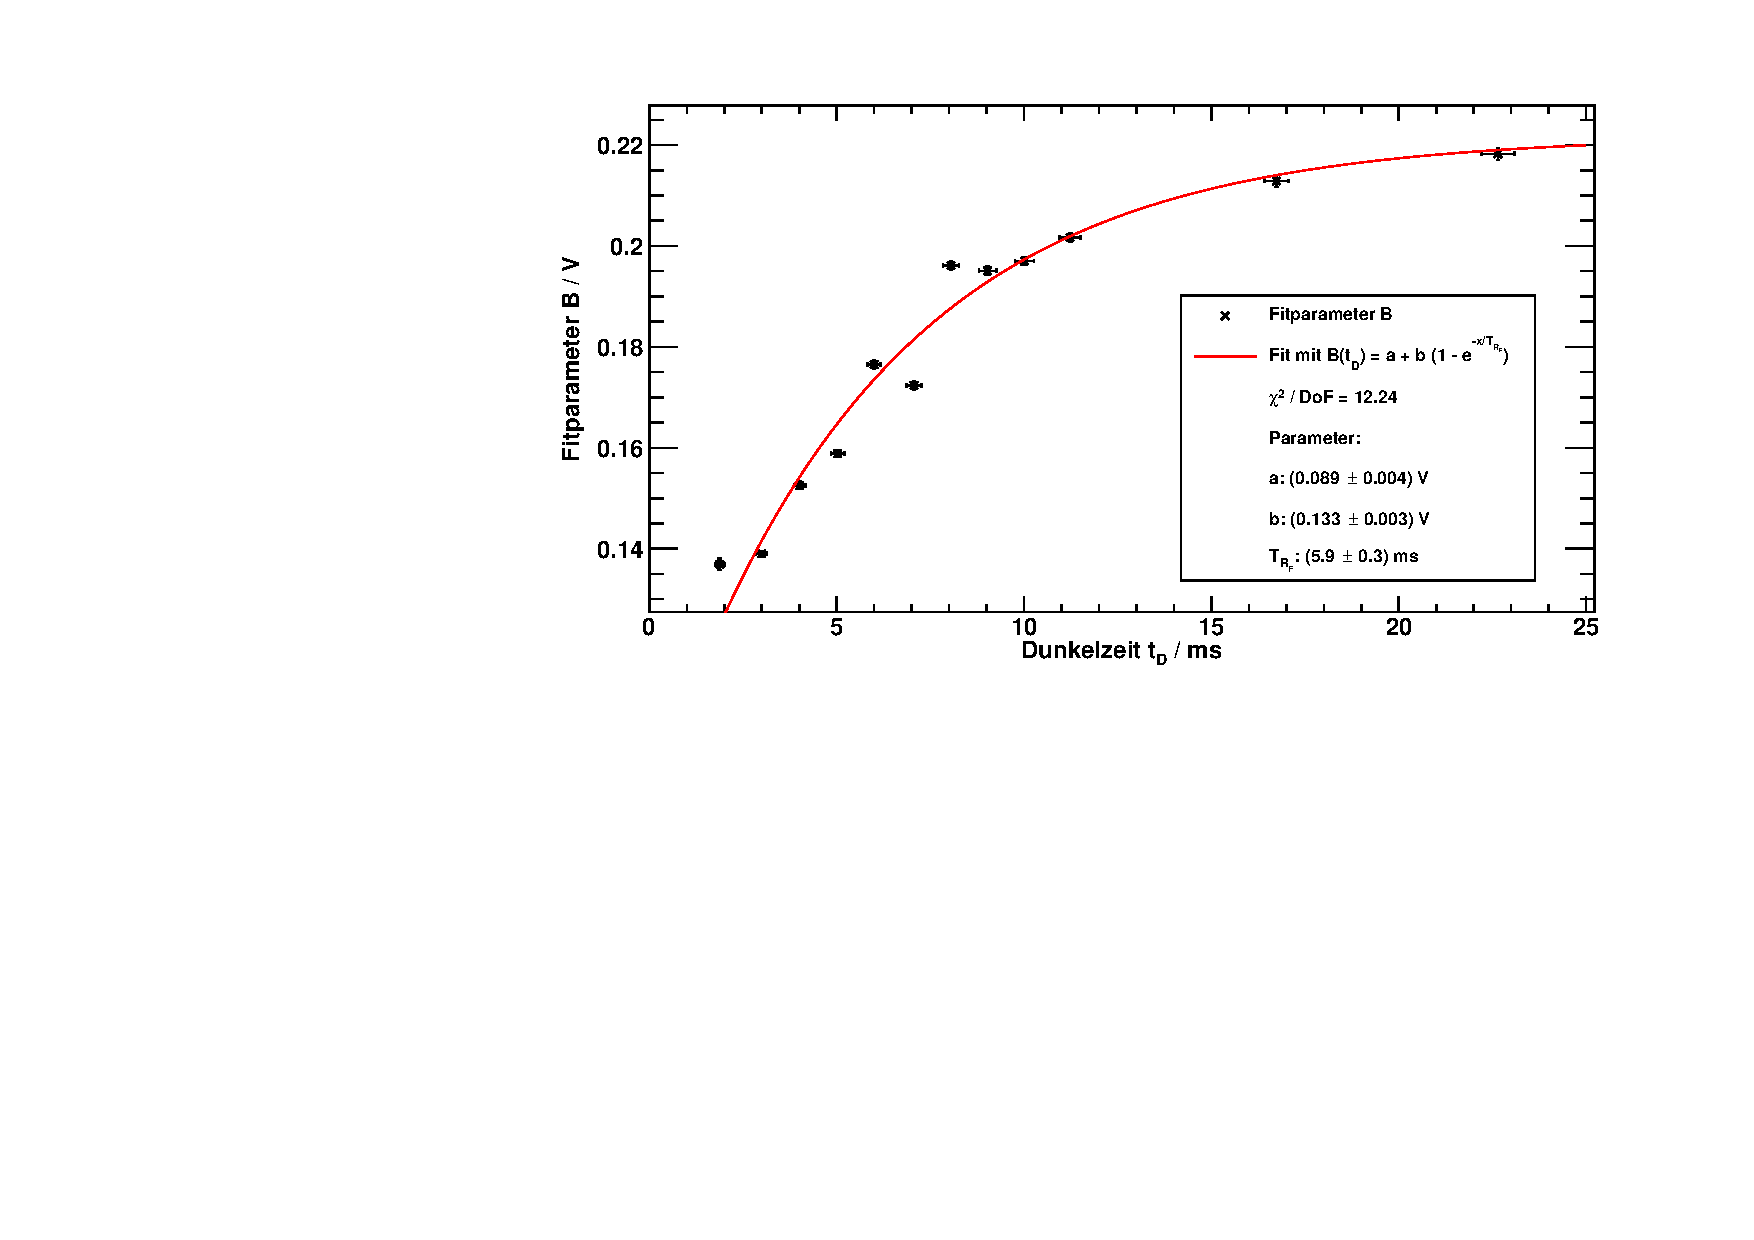
\includegraphics[width=\textwidth]{../img/BFit.pdf}
    \caption{Startwerte der gefitteten Exponentialfunktionen.}  
\end{figure} 
  
\end{frame}